\section{Colorizer Robot}
Again, text communications gets in the way of collaboration in some aspects. When working between several people it is sometimes necessary to talk about some aspect of the work they disagree in. In plain text, when there are more than two collaborators, there is no \textbf{way to know who edited what}, so those kind of issues can't be addressed personally. A robot is needed in order to know when and what changes are being made.

\label{subsec:color_soa}
\subsection{State of the Art}
In Wave it is possible to see who has participated in a blip as shown in Figure \ref{fig:participants}, but it is \textbf{not possible to see exactly what that participant has modified} what part of the document.
\begin{figure}[H]
  \center
    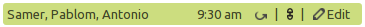
\includegraphics[keepaspectratio, scale=0.7]{Media/Captures/Wave/Participants.png}
  \caption{Blip Participants in Apache Wave}
  \label{fig:participants}
\end{figure}
The other thing Wave does to try to keep people informed on when changes happen, is to highlight the changes that just happened and write the author's name next to it, as shown in Figure \ref{fig:participants2}. The problem is it is not permanent, so you only realize of the change if you were already looking at the content being changed.
\begin{figure}[H]
  \center
    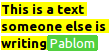
\includegraphics[keepaspectratio, scale=0.7]{Media/Captures/Wave/Participants2.png}
  \caption{Change Highlighting in Apache Wave}
  \label{fig:participants2}
\end{figure}
Also, this extension is heavily inspired in Pads, services like PiratePad, Etherpad, TitanPad and many others, that offer an online collaboration tool that allows to concurrently write plain-text documents. They show a specific color for each participant to quickly see who edited what. TitanPad in Figure \ref{fig:titanpad}, even though not the only, has the capability to show a timeline and revisit past states of the Pad, so no information is lost even after being modified.
\begin{figure}[h]
  \center
    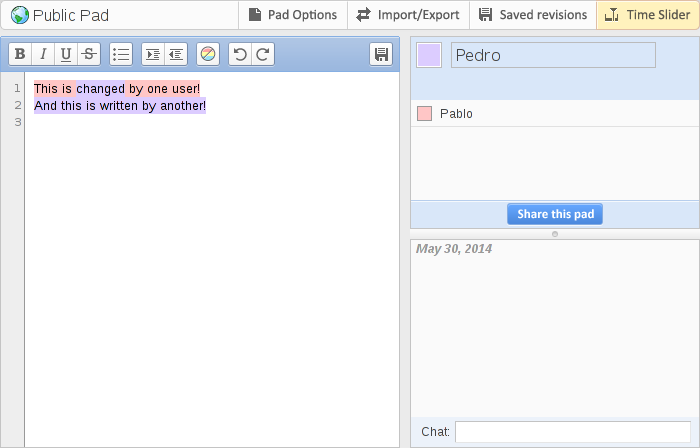
\includegraphics[keepaspectratio, scale=0.4]{Media/Captures/Soa/TitanPad.png}
  \caption{TitanPad}
  \label{fig:titanpad}
\end{figure}

\subsection{Results}
This extension, in the shape of a robot, goes around that problem by assigning a color to each participant, and painting the background of the text that participant edits. The result can be seen in Figure \ref{fig:colorizer_editions}. It also keeps track of who has each color and puts it in a blip under the main blip of the wave, as seen in Figure \ref{fig:colorizer_editors}. It is also possible to get around the colorizing of any given blip by starting it with \verb|@Robot clear annotations|, being ``Robot'' the actual name of the robot that it was registered with.\\[.2cm]
\begin{figure}[H]
  \center
    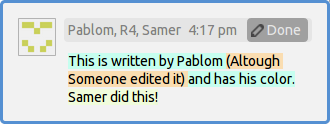
\includegraphics[keepaspectratio, scale=0.8]{Media/Captures/Extensions/Colorizer/ColorizerEditions.png}
  \caption{Colorizer Robot Colors}
  \label{fig:colorizer_editions}
\end{figure}
\begin{figure}[h]
  \center
    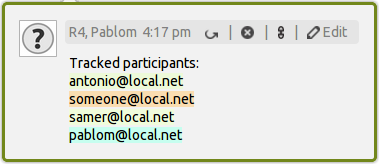
\includegraphics[keepaspectratio, scale=0.7]{Media/Captures/Extensions/Colorizer/ColorizerEditors.png}
  \caption{Colorizer Robot Tracking Participants}
  \label{fig:colorizer_editors}
\end{figure}
The way to make the background of the text be of a specific color is by changing the annotations of the document. Annotations in Wave are tags affecting a range of text and altering its properties, but they don't affect the text itself. Annotations are also able to be transmitted through the Federation Protocol. Every annotation is defined by a name (What it does), a range (What characters of text it affects), and a value (What value should that annotation take on that range). There are annotations for text size, links, language, among other. For this robot specifically the annotation \verb|style/backgroundColor| is the one being set in the changed text.\\[.2cm]
The way to know when the changes happen is by subscribing th the DocumentChanged event explained before. This event will be triggered anytime anyone modifies the text.\\[.2cm]
\begin{figure}[H]
  \center
    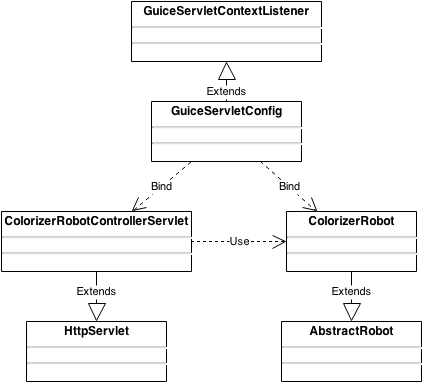
\includegraphics[keepaspectratio, scale=0.5]{Media/Diagrams/Robot/Colorizer.png}
  \caption{UML Class Diagram, Colorizer Robot}
  \label{fig:colorizer_diagram}
\end{figure}
That only leaves one task left: The DocumentChanged event tells us the document has changed, but not what part changed or how it changed, so it is up to us to extract that information. To achieve it Google's google-diff-match-patch, a Java library that is able to extract the difference between two chunks of plain text. Every time the document is changed, the difference with the last version is calculated, and the new content is attributed to the participant that changed it.\\[.2cm]
Figure \ref{fig:colorizer_diagram} represents the class structure of the Colorizer Robot. The HttpServlet is the responsible of receiving the communication from the Wave Protocol. The ColorizerRobot sets up the OAuth authentication with the token received when registering the robot. Also, thanks to the AbstractGadget class it is registered to receive all the events. The GuiceServletConfig binds the necessary dependencies together.
\begin{figure}[H]
  \center
    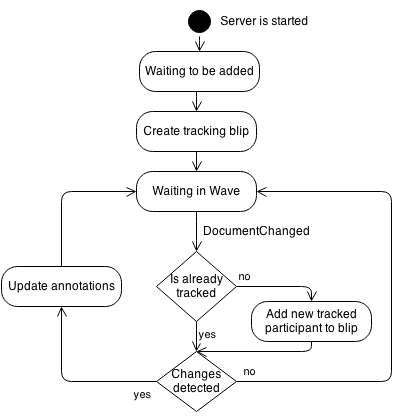
\includegraphics[keepaspectratio, scale=0.65]{Media/Diagrams/Robot/RobotActivity.png}
  \caption{UML Activity Diagram, Colorizer Robot}
  \label{fig:colorizer_activity_diagram}
\end{figure}
Figure \ref{fig:colorizer_activity_diagram} shows the behaviour of this robot in time, disregarding the aspects of the robot registration. Once the server is started, it is ready to be used as a robot and added as a participant to the wave. When it is added, the first thing done is creating the blip for tracking the participants that have acted. When the blip is created, it will start listening for Document Changed events. When each of those events is received, the robot will check if the participant that generated the event is already being tracked, and add it otherwise. The Document Changed event is triggered also when the document is changed by an equivalent one, so the difference of both documents has to be calculated. Annotations are updated according to the participants and changes. Afterwards, it goes back to waiting to another Document Changed event.

\subsection{Conclusions and Future Work}
This extension, as said before, uses an API for diff calculation that works with plain text. That means changes on annotations are not detected. Also, diff detection can be problematic in some specific cases. The difference between two documents is always computed correctly, but as the library does not have information on where the text changed, and it is not possible to extract that information from within the robots API, it will sometimes attribute a change to a wrong position of the text. For example: We have the string ``abc'', and a participant decides to add a new ``b'' to the left of the already existing ``b''. The end result would be ``abbc'', where the first apparition of the letter will be the change from the last version of the text. But because of how the diff calculation is made, the library will come up with the result that the difference between those two texts is the ``b'' on the right and the robot will put the background color in the wrong character. This small example can be extrapolated to more complex and problematic cases.\\[.2cm]
Wave, thanks to the federation protocol and the deltas, is able to keep track of all the history of the modifications in the document. Also because of deltas, changes can be attributed to a participant with little overhead, as opposed to calculating the difference every time a change is made. With past states it would be possible to reliably go back in history and review what happened. \textbf{Implementing this feature at a Wave protocol level} would definitely be advantageous.
